\section{Overview}
\label{sec:overview}

\subsection{Background of NUMA Architecture}

What type of issues for NUMA performance? 
There are three challenge: remote accesses, interconnect congestion, node imbalance. 

What is the overhead of remote accesses? Around twice of performance difference. 

What is the interconnect congestion? 

\subsection{NUMA Support Inside OS}

Operating System provides some NUMA support inside. The most common approach is to allocate the memory from the local node. However, this approach cannot guarantee to be optimal due to multiple reasons. First, it won't work for producer-consumer model, where the memory will be utilized by threads that are not in the same node. This is actually very common, especially for the main thread. Second, it does not work when cores on different processors have to be used, if the application utilizes more physical memory of one node, or if threads are migrated later. Third, it requires the user-level memory manager support. Otherwise, an deallocated object can be allocated to threads running on the other node, causing many remote accesses. 

Besides this, Operating System typically provides another memory policy where the memory will be allocated in an interleaved way. Also, OS provides different system calls that allow users to specific the memory policy, move memory, and schedule the threads. However, it is not designed for a specific applications, but providing interface that allows programmers to customize for their specific application.   


\subsection{Basic Idea of \NA{}}
\NA{} aims to reduce remote accesses, and balance the workload between different hardware nodes. It also aims to utilize the hardware support, such as huge page, to improve the performance. It further includes the following components as described in the following. 

\begin{figure*}[h]
\begin{center}
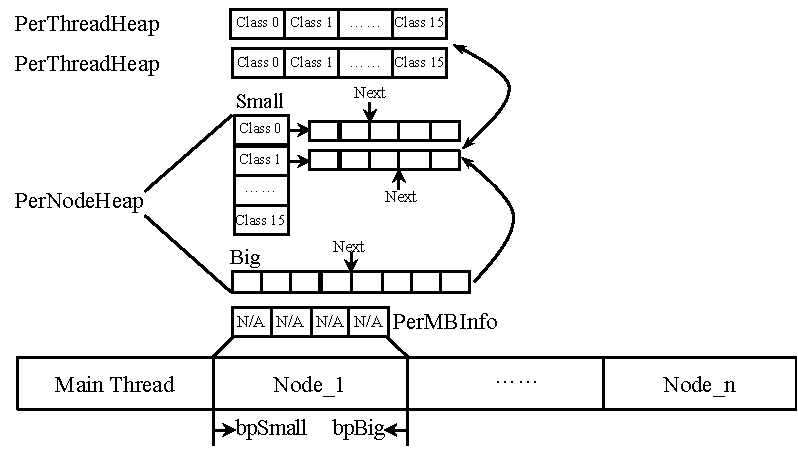
\includegraphics[width=0.8\textwidth]{figure/heaplayout}
%\includegraphics{figure/overview2}
\end{center}
\vspace{-0.1in}
\caption{Overview of \NA{}.
\label{fig:overview}}
\vspace{-0.1in}
\end{figure*}

\paragraph{Topology Aware Task Assignment} Due to the importance of task scheduling to the memory locality, \NA{} designs a topology-aware task assignment, which builds the basis for its memory management. More specially, \NA{} will bind every thread to a  memory node, and balance the workload among different nodes. At first, \NA{} will recognize the core-to-processor relationship, and then proposes a topology-aware task scheduling, which is similar to TBB-NUMA~\cite{Majo:2015:LPC:2688500.2688509}.  After that, every thread will be pinned to a specific node during its creation time, in order to avoid unnecessary performance lost caused by the thread migration. Note that a thread is pinned to a node, instead of a core, which still allows the OS scheduler to perform the load balance. \NA{} assigns threads to nodes with  a round-robin way, which ensures that each processor will have a similar number of threads, and therefore a similar workload.

\paragraph{NUMA-Aware Memory Allocation} \NA{} utilizes the huge address space of 64-bits machine to ensure the locality of any memory block. \NA{} obtains a big chunk of memory from the underlying OS initially, and then divides it to multiple chunks with the same size. Each chunk will be bound to a specific memory node with the NUMA API support. Therefore, the physical node information could be obtained from the virtual address directly, by checking the distance from the starting address of the heap. Since every thread is already pinned to a specific node, its allocations could only be satisfied from  its local node. \NA{} designs the per-node heap to hold objects that were allocated by a local thread but deallocated by a remote thread. If an object is deallocated by a local thread, it will be placed into the per-thread heap of the current thread. \NA{} eliminates the usage of locks for such deallocations.      

\paragraph{Interleaved and Blockwise Allocation  for Shared Objects} Based on our observation, most existing profiler identified the NUMA performance issues that are related to shared objects~\cite{}. If an object is not shared between multiple threads, most existing allocators will allocate such objects from the local node, causing no performance issue.   the main thread typically prepares the data for all of its children threads. That is, it is very likely that most objects allocated from the main thread will be shared by most threads. Therefore, it will cause the load imbalance issue, if all objects from the main thread are allocated from the node that the main thread is running on. Also, it could also introduce significant number of remote accesses, since not all threads could run on the same node.  

%\paragraph{Children Threads:} For normal threads, it is better to allocate the memory from the local node, in order to reduce remote accesses. But existing allocators have an issue to handle remote frees that the deallocation thread is not the same as the allocation thread~\cite{Aigner:2015:FML:2814270.2814294}. They tend to place freed objects into the current thread, such as TCMalloc~\cite{tcmalloc} or jemalloc~\cite{jemalloc}, no matter where these objects are allocated from.  However, this could cause remote accesses. In order to solve this issue, \NM{} proposes an information-computable design, as shown in Figure~\ref{fig:overview}. Basically, \NM{} utilizes the fact of 64-bit address space, where machines have extremely large amount of virtual address. Basically, \NM{} requests 32 TB virtual address at one time, and then divides it to multiple spans based on the number of nodes. For each span, \NM{} binds the memory to a specific node through \texttt{mbind} system call. Therefore, \NM{} is able to recognize the physical location by the address. During the deallocation, \NM{} will actually return a remote object to its owner, and only return the objects from the current node to the current thread's PerThreadHeap. 


\paragraph{Automatic Huge Page Support:} The default huge page support is not good for the performance~\cite{}. It also may have some harmful impact on the performance. However, if the huge page is utilized very well, the application's performance can be improved dramatically. The underlying reason is that it will have less TLB misses, since one TLB entry will cover a larger range of memory, such as 2MB instead of 4KB. Based on a simple test, using the TLB could improve a simple test case more than 10\%, without any other changes. To taking advantage of this benefit, each PerNodeHeap is further divided into two parts, where small objects will be allocated from the beginning and will be allocated using small pages, while big objects will be allocated from the end of the heap using huge page (2MB). We believe that this mechanism balances the performance and memory consumption.   

\paragraph{Reutilization of Big Objects:} Existing allocators will handle big objects different with small objects, which will be allocated from the OS directly. When these objects are freed, they will be returned to the OS directly by invoking \texttt{munmap} or \texttt{madvise}. This mechanism was designed to reduce memory consumption. However, this mechanism will invoke a lot of unnecessary overhead. Taking an object with the size of 1 MB as the example, this object includes 256 pages (4KB). Therefore, the overhead includes returning 256 pages to the OS (by modifying the page table entries of 256 pages), and then 256 page faults when this is returned. More importantly, cache lines of these 256 pages should be reloaded from the memory after allocating these physical pages. \NM{} aims to reduce such overhead based on a simple assumption: if the application is requesting memory, then big objects should not be returned to the OS to avoid such overhead. In fact, \NM{} proposes to utilize these big objects for small objects. Due to this design, \NM{} actually utilizes 1MB as the basic unit, and then allocates 1MB for small objects on demand. 

\paragraph{Node-local Metadata:} \NM{} designs the metadata meticulously, which will be always allocated in the same node. Such metadata includes the PerMBInfo, freelists for different size classes, and freelists for big objects. PerThreadHeap's metadata will be also allocated in the local node as well, which has been assigned to a specific node during thread creation. 


 